\chapter{提案手法}
\label{proposed}

本章では提案手法について述べる.

\section{概要}

本研究では, 人間の状態とモビリティの経路を再現するシミュレータープログラムを開発し実験を行う.
なお, シミュレータープログラムの作成にあたっては以下について仮定を行った.

\begin{itemize}
    \item シミュレーター上での自動車は全てレベル5の完全自動運転ができる物とする
    \item 歩行者や, 自動運転非対応者などは考慮していない
    \item シミュレーターでは予め決められた幹線道路及, 環状線などのバイパス道路のみを考慮し, それ以外の道に関しては考慮しない
    \item 人間の目的を正確に推定するコンピューターシステムもしくはセンサーなどは実在しているものとする. 
\end{itemize}

\subsection{路線網の正規化}

本研究では実際の道路網を参考に仮想の道路網モデルを構築した.
選び出したルートの正則化を行った。実際の地図上にある道路のPOLYLINEデータは道路路線上の点の集合体であり, これを結んだ線分として記録されている. しかし, DQN機械学習モデルでは限られた次元数の行列データしか扱うことができず, そのままではDQNに学習させることができない。
そこで、本研究では、1つのPOLYLINEを交差点毎に分解し交差点に挟まれた1区間を行列の1次元に表し1つの要素とした.
この場合, 区間の距離に関わらず1次元の要素として表すため距離情報が失われる. 従って, ここでは距離を通過難易度dとして環境定義することで距離データを失わないようにした.



\begin{figure}[H]
    \centering  % 図を真ん中に配置
    \includegraphics[clip,width = 13.0cm]{assets/MAP_1.eps}
    \caption{地図上の道路を選択する}  \label{sample}
\end{figure}


\begin{figure}[H]
    \centering  % 図を真ん中に配置
    \includegraphics[clip,width = 13.0cm]{assets/MAP_2.eps}
    \caption{交差点箇所にマークをつける}  \label{sample}
\end{figure}


\begin{figure}[H]
    \centering  % 図を真ん中に配置
    \includegraphics[clip,width = 13.0cm]{assets/MAP_3.eps}
    \caption{地図を省いて路線網だけにした図}  \label{sample}
\end{figure}


\begin{figure}[H]
    \centering  % 図を真ん中に配置
    \includegraphics[clip,width = 13.0cm]{assets/MAP_4.eps}
    \caption{曲線部分を省き直線化する}  \label{sample}
\end{figure}


\begin{figure}[H]
    \centering  % 図を真ん中に配置
    \includegraphics[clip,width = 13.0cm]{assets/MAP_5.eps}
    \caption{区間の長さを等しく正方形にする}  \label{sample}
\end{figure}


\subsection{選択した道路のデータ化}

選択した道路の線形をPostgreSQLにてデータ化を行った. なお, この実験で使用したPostgreSQLには地理情報を扱う拡張であるPostGISをインストールしている.
データ化した内容は, 道路網の一定間隔の座標である. この座標同士を結ぶ線分をPOLYLINE型で記憶し路線名や道路が受け入れることのできる車の第数=Capacityを定義した.

\begin{lstlisting}[caption = 路線データを表すクエリーの例, label = program1]

/*
    テーブル構造の定義
*/
CREATE TABLE geodb_catp_yokohama (
    id                  serial PRIMARY KEY,
    route_name          VARCHAR (100),
    has_spot    VARCHAR (20),
    capacity            INTEGER
);

/*
    線地理情報を記録するPOLYLINE型のカラムを追加
*/
SELECT AddGeometryColumn ('public', 'geodb_catp_yokohama', 'geometry_data', 4326, 'LINESTRING', 2);

/*
    道路の線形を表すデータのレコード
*/
INSERT INTO geodb_catp_yokohama (route_name, has_spot, capacity, geometry_data)
VALUES ('K1',
        'none',
        200,
        ST_GeomFromText('LINESTRING(139.633639 35.445911, 139.632631 35.447126 ...... 139.632323 35.472085)', 4326));
\end{lstlisting}

%%% Local Variables:
%%% mode: japanese-latex
%%% TeX-master: "../bthesis"
%%% End:
